\chapter{Development documentation}

The software is a locally-run web application. It consists of three principal parts that ensure its proper functioning: the database, back end and
front end. Their interactions are outlined in Figure \ref{fig:architecture}.

\begin{figure}[!h]
\centering
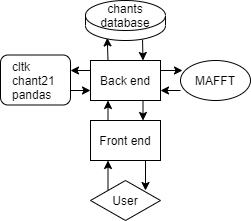
\includegraphics{ddocs_layout}
\caption{A high-level overview of the application's architecture.}
\label{fig:architecture}
\end{figure}

The database stores the data used by the application. The data it contains do not impact the functionality of the application. It can be added
to or removed from, as long as the added data follows the schema. It is even possible to have multiple databases and use the one that is currently needed.

The back end is the part of the application that takes care of the internal logic. It pulls data from the database and adds new ones. It performs calculations
that would be too compute-intensive for the front end. The back end is interacted with via its API: anyone can make an appropriate http request
to a specified URL and the back end returns the corresponding response.

The front end is the user-facing interface. Its main function is to display data returned by the back end. It can also perform some lighter calculations.
The user interacts with the front end via a web browser.

In the following sections, we will describe the proper functioning of each part in more detail.

\section{Data}

In this application, we use SQLite\footnote{\url{https://www.sqlite.org/}} as our data\-base technology. It is a lightweight and self-contained database engine,
which makes it easy to work with. It is the predefined database for the back end technology and comes with several drawbacks, such as a relatively low performance.
However, as our use case is not data-heavy, we have not opted for a different technology since we prefer flexibility over performance.

Our database consists of a single table \verb|chant|. The fields of one entry are described in Section \ref{section:db_fields}. Its schema is shown
in Figure \ref{fig:schema}.

\begin{figure}[!h]
\centering
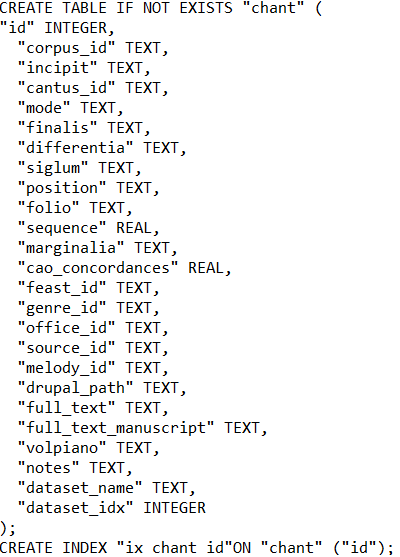
\includegraphics{ddocs_schema}
\caption{Schema of the \emph{chant} table.}
\label{fig:schema}
\end{figure}

The last two fields, \verb|dataset_name| and \verb|dataset_idx| determine to which data source the row belongs. Data source is the main grouping criterion
for data in this application. The user may select multiple data sources for comparison. The expected amount of data in each data source is in the order
of thousands of entries at most. We chose to store all data in one database, as opposed to e.g. having one database for each data source, as the expected
scale of data does not justify working with a more complex scheme.

\section{Back end}

The Python programming language is often used in academic contexts. It allows for rapid development and great flexibility. Python applications are easily
integrated with other programs, which we need for MAFFT integration. There are also many libraries available for working with data in general (e.g. \verb|pandas|)
and for our specific data (\verb|cltk| for working with Latin texts, \verb|chant21| for working with chants). Because of these properties, we decided to use Python
for our application's back end.

The back end uses the Django framework.\footnote{\url{https://www.djangoproject.com/}} Django is a Python web framework enabling developers to create web
applications quickly, having abstracted away the most tedious of web development aspects.

Django programs consist of one or more logical units called \emph{apps}. An \emph{app} is a self-contained program providing some related functionality. Thanks
to Django's modularity, an \emph{app} can be plugged in into many projects without the need to always rewrite it. Our application only uses one \emph{app},
\verb|melodies|, which provides REST API to other programs.

% the app only contains one app, melodies
The app only contains one app, \verb|melodies|, which provides the API for other applications. The app uses the module \verb|core| providing the essential
computations.

To ensure proper integration with the front end, it is necessary to include allow front end's server to interact with the back end. This is done by
including front end's URL in the array \verb|CORS_ORIGIN_WHITELIST| in the \verb|settings.py| file. In the event of deployment, the URL
would need to be changed appropriately.

\subsection{REST API}
\label{section:api}

The \verb|melodies| app provides API that offers other programs a way of interacting with it. It is done in the form of web requests to a specific URL. The requests
can be either GET or POST requests. GET requests do not contain any additional data; the response returned always depends only on the state of the application. On
the contrary, POST requests contain data that the application takes into account when constructing the response.

Table \ref{table:api} summarizes the API provided by the application. The API is described into more detail below.

\begin{longtable}{| p{.24\textwidth} | p{.09\textwidth} | p{.18\textwidth} | p{.39\textwidth} |} 
%\begin{center}
%\begin{tabular}{| c | c | c | c |} 

 \hline
 Endpoint & Method & POST fields & Description \\
 \hline
\emph{api/chants/}                & POST & \verb|dataSources|, \verb|incipit|, \verb|genres|, \verb|offices| & Returns a list of chants filtered by their data source, incipit, genre and office\\
\emph{api/chants/\textless pk\textgreater} & GET  &                                                          & Returns the chant with the ID \verb|<pk>|\\
\emph{api/chants/sources}         & GET  &                                                                   & Returns a list of all data sources currently present in the database with their name and index\\
\emph{api/chants/upload/}         & POST & \verb|file|, \verb|name|                                          & Uploads \verb|file| to the database as a new data source and gives it the specified \verb|name|\\
\emph{api/chants/export/}         & POST & \verb|idsToExport|                                                & Returns a CSV file containing the chants with the specified IDs\\
\emph{api/chants/create-dataset/} & POST & \verb|idsToExport|, \verb|name|                                   & Creates a new data source from the chants with the specified IDs and gives it the specified \verb|name|\\
\emph{api/chants/align/}          & POST & \verb|idsToAlign|, \verb|mode|                                    & Takes chants with the specified IDs and aligns them according to \verb|mode|\\
 \hline

%\end{tabular}
%\end{center}
\caption{API of back end.}
\label{table:api}
\end{longtable}

\begin{itemize}

\item \textbf{api/chants/} The POST request must contain the fields as specified in Table \ref{table:api}. \verb|dataSources| is a list of indices of allowed data sources as stored
in the database. \verb|incipit| is a string that must be present as a substring in the \emph{incipit} field in each of the returned entries. \verb|genres| and \verb|offices|
are lists of strings, where each string is an identifier of a genre or an office, as seen in Attachment XX. Each returned entry must have its genre be an element of \verb|genres|
and its office be an element of \verb|offices|. The response is a list of all entries in the database satisfying these constraints.

\item \textbf{api/chants/\textless pk\textgreater} The application looks for a chant with the ID \verb|pk| in the database. It returns an error if no such entry exists. If it does,
it returns a JSON object with the following keys: \emph{db\_source}, which is the entry as stored in the database, \emph{json\_volpiano}, which is the chant processed in
such a way that its melody and text are easy to display in an HTML template, and \emph{stresses}, a list of stressed syllables corresponding to the chant's text, if it
can be computed.

\item \textbf{api/chants/sources} The response is a JSON object with one key, \verb|sources|. Its value is the list of pairs representing the data sources currently present in
the database. The first value of each pair is a data source index and the second one is its name.

\item \textbf{api/chants/upload/} The POST request must contain a CSV file as specified in Section XX in the field \verb|file| and a string \verb|name|. The data in the file
will be uploaded directly to the database as a new data source with the given name. Some values may be changed before inserting the data in the database, namely the columns
\emph{id}, \emph{dataset\_idx}, and \emph{dataset\_name}, if the file contains them. The response is a JSON object with the keys \emph{name}, the name of the new data
source, and \emph{index}, the index assigned to it.

\item \textbf{api/chants/export/} The POST request body must contain the field \verb|idsToExport|. It is a list of integers representing the IDs of the chants to be exported. If
an ID does not correspond to any chant in the database, the ID will be excluded. The response contains a CSV file with its entries being the corresponding chants, formatted
as outlined in Section XX.

\item \textbf{api/chants/create-dataset/} The POST request must contain a list of chant IDs in the field \verb|idsToExport| and a string in the field \verb|name|. The chants
that correspond to the IDs will be duplicated in the database, given new IDs and assigned to a new data source with the name as specified in the field \verb|name|.
The response is the same JSON object as in the \emph{upload} API, containing the keys \emph{name} and \emph{index}, the name and index of the newly created data source.

\item \textbf{api/chants/align/} The POST request contains two fields. \verb|idsToAlign| is the list of chant IDs we want to align. \verb|mode| is the mode of alignment we chose.
Its values can be \emph{syllables}, which is the word-based alignment, \emph{full}, the alignment on pitches, or \emph{intervals}, the alignment on intervals. If the
value is not one of those, the request will return an error. The response is a JSON object with the following keys: \emph{chants} is an object representing the
aligned melodies along with their texts, easily renderable by an HTML template. \emph{errors} contains a list of chant IDs of the chants that could not be aligned for
various reasons. \emph{successes} contains an object that describes the chants that have been successfully aligned: \emph{sources} are their original sources (i.e.
siglum, folio and position), \emph{ids} the IDs as stored in the database, \emph{volpianos} the melodies as given by the alignment algorithm, and \emph{urls} the
values in the \emph{drupal\_path} field of the database.

\end{itemize}

\subsection{Core}

\verb|core| is the Python module that contains essential functionality ensuring the proper behavior of the application, e.g. the implementation of alignment,
MAFFT integration, and others. Figure \ref{fig:core} outlines the classes provided in the submodule and how they interact. The classes' functionality
is described below.

% MAFFt dat mimo core
% farebny hranaty ramcek pre core
% mozno aj napisat cltk
% prehodit api a core sekcie - a rovno napisat ktore api calls to pouzivaju
\begin{figure}[!h]
\centering
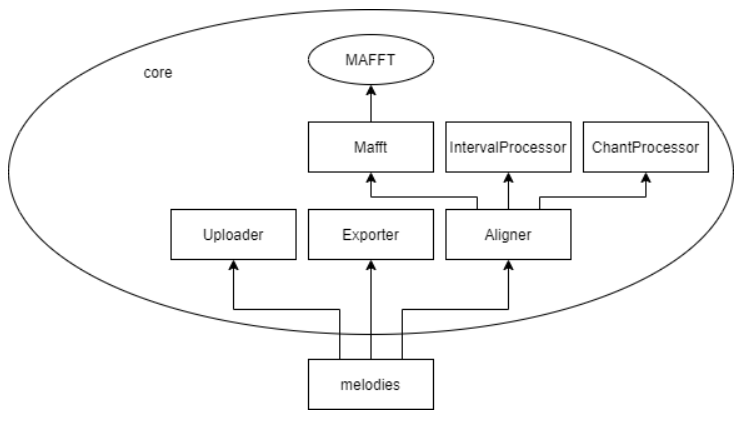
\includegraphics[scale=0.9]{ddocs_core}
\caption{Outline of the classes contained in \emph{core} and their interaction. An arrow from A to B indicates that A depends on B.}
\label{fig:core}
\end{figure}

% vyraznejsie nadpisy pre triedy - napr subsubsection
\begin{itemize}

\item\textbf{Exporter.} The class contains one method, \verb|export_to_csv|. It takes as an argument a list of chant IDs contained in the database. It returns
a response with a file with the corresponding database entries formatted as CSV.

\item\textbf{Uploader.} The class defines one method, \verb|upload_csv|. Its arguments are a \emph{pandas}\footnote{\url{https://pandas.pydata.org/}} dataframe, containing
data columns as described in Section \ref{section:db_fields}, and a dataset name. The method inserts the data into the database, ensuring that no duplication 
of IDs occurs. Input sanitization is done by the Django framework.

\item\textbf{ChantProcessor.} The class contains functionality for working with Latin texts and with melodies encoded as Volpiano. The method \verb|get_syllables_from_text|
takes a string of Latin text and returns the text syllabified: the returned value is a list, each of whose elements represents a word of the text, and each word
is a list of strings representing the syllables in that word. To syllabify the text, we use the module \verb|cltk|,\footnote{\url{http://cltk.org/}} which facilitates
working with classical languages, including Latin.

Some parts of the application require the encoded melody to contain no \verb|-| characters. Instead, they assume that ends of words are marked with a tilde (\verb|~|) and ends of
syllables with a pipe (\verb=|=). The method that converts proper Volpiano-encoded melody to this processed format is the method \verb|insert_separator_chars|.
The equivalent of syllabifying text for melodies is \verb|get_syllables_from_volpiano|. It takes a melody encoded as a processed Volpiano string (with \verb|~| and \verb=|=
instead of \verb|-|.). It assumes that the
melody contains a clef at the first position and a bar line at the last position, which is the proper way of encoding melodies according to the Volpiano
protocols.\footnote{\url{https://cantus.uwaterloo.ca/sites/default/files/documents/2.\%20Volpiano\%20Protocols.pdf}} The method returns a list whose elements represent words,
and each word is a list of strings representing syllables (equivalent to the syllabifying method for text). Examples of using these functions are shown in Figure \ref{fig:syl_text}
and Figure \ref{fig:syl_volpiano}.

\begin{figure}[!h]
\centering
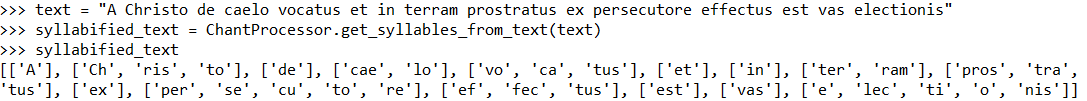
\includegraphics[scale=0.6]{ddocs_text-to-syllables}
\caption{Example of dividing Latin text into syllables using \emph{ChantProcessor}.}
\label{fig:syl_text}
\end{figure}

\begin{figure}[!h]
\centering
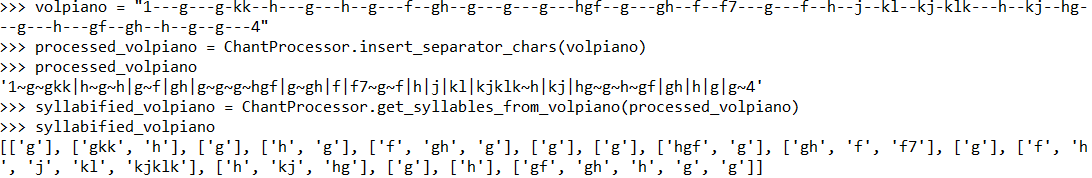
\includegraphics[scale=0.6]{ddocs_volpiano_to_syllables}
\caption{Example of dividing a melody encoded as Volpiano into syllables using \emph{ChantProcessor}.}
\label{fig:syl_volpiano}
\end{figure}

The method \verb|get_stressed_syllables| takes a Latin string as input and returns a list whose elements represent words, where word is a list of 0s and 1s,
a 0 representing an unstresed syllable and a 1 representing a stressed one. To calculate the stressed syllables, we use the module \verb|cltk|. However, 
its stress recognition is not completely accurate, therefore this method may also return incorrect results. However, no other functionality depends on
the results of the stress calculation. The function is shown in use in Figure \ref{fig:syl_stress}.

\begin{figure}[!h]
\centering
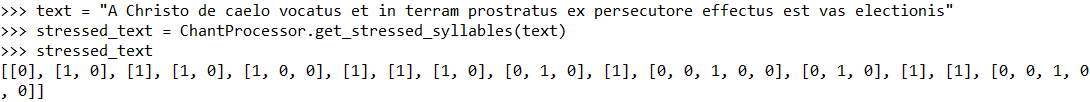
\includegraphics[scale=0.6]{ddocs_syllables-stressed}
\caption{Example of finding the stressed syllables of a Latin text using \emph{ChantProcessor}.}
\label{fig:syl_stress}
\end{figure}

\item\textbf{IntervalProcessor.} The class provides tools to work with the interval representation of a melody. It contains two methods, \verb|transform_volpiano_to_intervals|
and \verb|transform_intervals_to_volpiano|. \verb|transform_volpiano_to_intervals| takes a string representing a melody (it can be encoded either as dictated by the Volpiano protocol, or processed
to have its words separated by \verb|~|s and syllables by \verb=|=s for the purposes of alignment, see Section \ref{section:vol_preprocess}) and returns the same melody represented as intervals.
\verb|transform_intervals_to_volpiano| is its reverse: it takes a string representing a melody encoded by intervals and returns the Volpiano representation.
Figure \ref{fig:vol_intervals} shows how these functions are used.

\begin{figure}[!h]
\centering
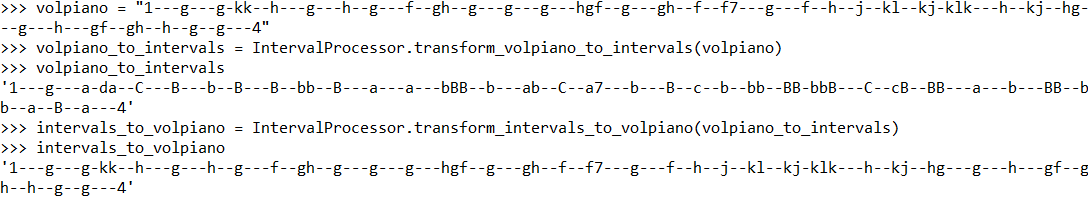
\includegraphics[scale=0.6]{ddocs_intervals}
\caption{Transforming a Volpiano-encoded melody into an interval representation and back.}
\label{fig:vol_intervals}
\end{figure}

\item\textbf{Mafft.} This class provides the interface for working with the MAFFT software.\footnote{\url{https://mafft.cbrc.jp/alignment/software/}} The software must be installed
on the computer that runs the application. On Windows systems, it is assumed that it is installed in a WSL instance.\footnote{\url{https://docs.microsoft.com/en-us/windows/wsl/}}
On other systems, it has to be installed natively.

An instance of the class encapsulates the action of aligning one set of data. It needs to have a specified input file, and, optionally, an output file, which can be set
via the methods \verb|set_input| and \verb|set_output|. If the user wishes to run the alignment with other options as specified in MAFFT's documentation, it can be done
using the method \verb|add_option|. The method \verb|add_volpiano| can optionally be used if the user does not want to provide their own file (however, its location must
still be defined) or wishes to add another sequence to align. MAFFT is only run by calling \verb|run_process|. The result of the alignment is retrieved using the methods
\verb|get_aligned_sequences| and \verb|get_sequence_order|, which return the aligned sequences and their headers, respectively, in the order of similarity.

\item\textbf{Aligner.} The class defines the methods to compute the three types of alignment, as described in Section \ref{section:chant_alignment}: \verb|alignment_syllables|,
which performs the word-based alignment; \verb|alignment_pitches|, computing the alignment of pitches; and \verb|alignment_intervals|, which return the alignment of 
intervals. All of them take as an argument just the list of IDs of the chants to be aligned and return a dictionary easy to work with in HTML templates.
% alignment_syllables nepouziva triedu mafft, ostatne ano - interval pouziva aj interval processor

\end{itemize}

\section{Front end}

For the front end, our application uses the Angular framework.\footnote{https://angular.io/} An Angular application
consists of components, which are small, relatively self-contained units exposing some functionality of the application (both appearance and behavior), and
services, providing means of sharing and manipulating data, e.g. the interaction with the back end. Both components and services should only contain
a small, logically contained set of functionality. This makes the application safe and scalable. Most importantly, the framework keeps track of the data
passed to it and updates the appearance dynamically.

This application contains several components and services that interact with each other. Figure \ref{fig:frontend-schema} shows a diagram of the front end architecture.
The elements in rectangles are components. Orange background, \emph{AppComponent}, represents the component encapsulating the entire application. Blue
background represents components that are always present on the page. A dotted arrow from component A to component B indicates that component A has component
B in its HTML template. The ellipses represent services. An arrow from a component or service A to service B means that element A uses service B.

The following sections describe each service and component in more detail.

% pridat do popisku co su obdlzniky etc
% vyfarbit podla toho na ktorej su stranke
% hruba farebna sipka "api calls"
\begin{figure}[!h]
\centering
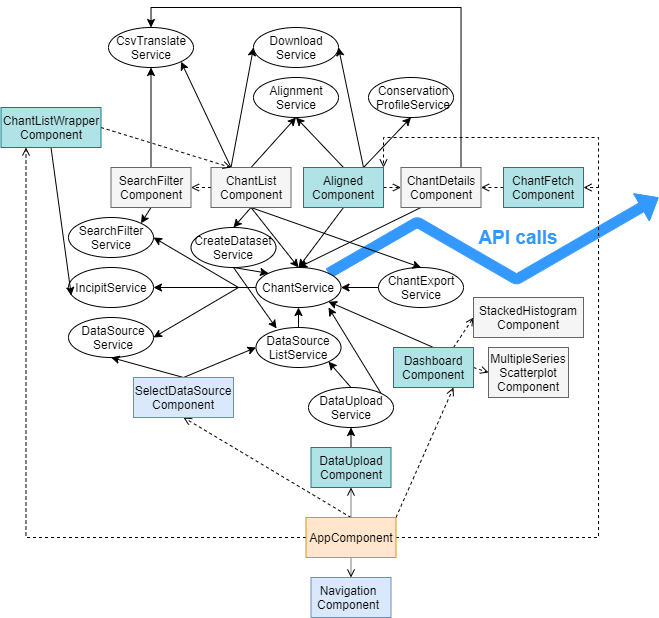
\includegraphics[scale=0.8]{ddocs_frontend-schema}
\caption{The architecture of the front end.}
\label{fig:frontend-schema}
\end{figure}

\subsection{Services}

% urobit z toho zoznam

\begin{itemize}

\item\textbf{ChantService.} This service is the service responsible for communication with the back end. It uses back end's API as described in Section \ref{section:api} to
obtain the desired data. The method \verb|getChant|, taking a single number as an argument, sends a request to the back end to retrieve the chant with 
the ID equal to the argument. The method \verb|loadData| uses the current values stored int \emph{IncipitService}, \emph{SearchFilterService}, and
\emph{DataSourceService} to obtain all chants adhering to the constraints; the method \verb|getList| provides the object where these results are stored.
The method \verb|getAlignment| takes a list of chant IDs and an alignment mode and makes a request to the back end to calculate the corresponding alignment.
\verb|getDataSources| obtains all data sources currently present in the database. \verb|exportChants| takes as an argument a list of chant IDs and the 
corresponding API call returns a CSV file with their database entries. \verb|createDataset| creates a new data source from the chant IDs and name provided
to it. All arguments to these functions are passed as a part of a \emph{FormData}\footnote{https://developer.mozilla.org/en-US/docs/Web/API/FormData}
object.

\item\textbf{IncipitService.} The service stores the value of the incipit search query which is used when pulling data from the database. It provides two methods:
\verb|setIncipit| which changes the current value of the search query, and \verb|incipit| which returns a \emph{BehaviorSubject}\footnote{https://www.learnrxjs.io/learn-rxjs/subjects/behaviorsubject}
storing the value.

\item\textbf{SearchFilterService.} The service stores an object containing a list of allowed genres and a list of allowed offices which will be used for filtering
when retrieving data from the database. It provides two methods, \verb|setFilterSettings|, which changes the current value, and \verb|getFilterSettings|, returning
a \emph{BehaviorSubject} with the value.

\item\textbf{DataSourceService.} The service stores a list of indices of data sources we are currently using. The stored value persists throughout browser sessions.
The service has two methods, \verb|setSourceList|, which changes the value, and \verb|getSourceList|, which returns a \emph{BehaviorSubject} with the list.

\item\textbf{DataSourceListService.} The service stores a list of the data sources in the database as of the time of the last call to the back end's API. The list
is accessed by calling \verb|getAllSources|. The method \verb|refreshSources| retrieves the current list of data sources from back end.

\item\textbf{CreateDatasetService.} The service contains one method, \verb|createDataset|. It takes as an argument a list of chant IDs and a data source name and
ensures that it is sent to back end to be inserted into the database. Additionally, it calls \emph{DataSourceListService}'s \verb|refreshSources| to obtain the
most recent list of data sources.

\item\textbf{DataUploadService.} The service contains one method, \verb|uploadData|. It takes two arguments, a CSV file and a data source name. It passes these to \emph{ChantService}
to be inserted into the database and assures that the current data source list is correct by a call to \emph{DataSourceListService}.

\item\textbf{ChantExportService.} The service provides one method, \verb|exportChants|. Its argument is a list of chant IDs to be exported. The method returns a CSV
file with these chants.

\item\textbf{CsvTranslateService.} The service provides means to obtain a genre's or an office's full description given its identifier as stored in the database.
The descriptions are sourced from CSV files provided in CantusCorpus. They can be accessed via the methods \verb|getGenre| and \verb|getOffice|, both
taking the identifier of the genre or office as an argument. The service also contains the method \verb|getAllValues|, which takes as an argument either
the string \emph{genres} or \emph{offices}, and returns an object containing all values of the given type.

\item\textbf{DownloadService.} The service contains a single method, \verb|download|. It takes two arguments: \verb|blob|, which is the content of a file to
be downloaded, and \verb|filename|, the name of the file. Calling the method triggers the download of the file. The service is used in multiple situations.
It ensures the download of CSV files with exported chants, as well as the download of text files with the results of the alignment.

\item\textbf{AlignmentService.} The service stores the IDs of chants we want aligned and the algorithm using which they should be aligned. Both of these values persist
throughout browser sessions. The IDs can be changed or obtained by calling the setter and getter on \verb|idsToAlign|. The algorithm can be set via the method
\verb|setMode|, which returns 0 if the provided algorithm is correct and 1 otherwise; and retrieved with the method \verb|getMode|. The allowed algorithm values are
\emph{full}, \emph{intervals}, and \emph{syllables.}

\item\textbf{ConservationProfileService.} The service contains only one method called \verb|calculateConservationProfile|. Given a list of aligned melodies, as computed by the back end,
it calculates the conservation value for each position in each melody. It returns it in a form easy to work with in HTML templates.

\end{itemize}

\subsection{Components}

% screenshoty - moze byt viac komponentov v jednom komponente

\begin{itemize}

\item\textbf{AppComponent.} This component is the one always present on the page, encapsulating other components. It defines the global styles of the entire page.
The component displays \emph{SelectDataSourceComponent} and \emph{NavigationComponent}, which means they are always visible on the page. It further displays
components depending on the current URL, as indicated by the \verb|router-outlet| tag.

\item\textbf{NavigationComponent.} The component provides easy navigation to the app's main pages. It also enables the user to enter a query for searching
among the chants' incipits via the field in the top right corner. The \emph{home} button in the top left corner leads to the landing page.

\item\textbf{SelectDataSourceComponent.} The component exposes the interface to change the current selection of data sources. It contains a list of data sources
names, each next to a checkbox. The \emph{Save} button saves the current selection of data sources.

\item\textbf{ChantLlistWrapperComponent.} The component encapsulates \emph{ChantListComponent}. It reads the incipit search query from the current URL and
passes it to \emph{IncipitService}.

\item\textbf{ChantListComponent.} The component displays a list of chants from the current search results. The table contains a chant's incipit, source, genre, office, and
its data source. The checkboxes next to the incipits allow for the chants' selection. The component also provides the possibility to filter search
results, to export a selection of chants, to align a selection, and to create a new data source.

\item\textbf{SearchFilterComponent.} The component enables the user to select which genres and offices should be included in search results. It consists of
a set of checkboxes that determine whether a specific genre or office is allowed or not. The settings are saved using the \emph{Save} button.

\item\textbf{AlignedComponent.} The component displays results of alignment. It shows the aligned chants ordered by similarity in rows under each other. It
provides the means to hide and unhide text and headers, completely remove or collapse an alignment, rearrange the order, as well as highlight notes and
conservation profile. It also provides the possibility to export the results to a file.

\item\textbf{ChantFetchComponent.} The component encapsulates \emph{ChantDetailsComponent}. It reads chant ID from URL and passes it to \emph{ChantDetailsComponent}.

\item\textbf{ChantDetailsComponent.} The component displays the relevant information about a selected chant. It displays a melody with its text whose stressed
syllables are highlighted if possible.

\item\textbf{DashboardComponent.} The component displays several visualization of data from the current search selection. It preprocesses the data sent to
each of the visualizations.

\item\textbf{StackedHistogramComponent.} The component contains a histogram of data passed to it. We use the library \emph{d3js}\footnote{\url{https://d3js.org/}}
for the plot creation.

\item\textbf{MultipleSeriesScatterplotComponent.} The component shows a scatter plot of data passed to it. Again, we use the library \emph{d3js}.

\item\textbf{DataUploadComponent.} The component displays the interface for uploading a file to the database.

\end{itemize}

\section{Dependencies}

The software depends on several other programs for its correct functionality. For the back end, it is necessary to have Python installed. During development,
version 3.9.2 was used; it is not guaranteed that the application will work for lower versions. Additionally, the packages Django (version 3.1.7), pandas (version 1.2.3)
chant21 (version 0.4.6) and cltk (version 1.0.5) are required. It is also necessary to have the MAFFT software installed (version 7.470 or higher).

The front end is run on Angular version 11. It uses the library d3 (version 7.6.0) for visualizations.

